\section{Технический проект}
\subsection{Общая характеристика организации решения задачи}

Разрабатываемая программно-информационная система представляет собой настольное приложение, ориентированное на выполнение двух основных функций: генерацию карт нормалей по 2D-изображениям и интерактивную визуализацию этих карт в контексте имитации освещения. Цель системы — предоставить пользователю удобный и гибкий инструмент для анализа текстур и их освещённых свойств, применимых в игровой разработке и визуализации [21].

Особенностью разрабатываемой системы является её полная автономность: для использования программы не требуется подключение к сети Интернет, установка дополнительных серверов или сторонних сервисов. Все вычисления выполняются локально, на стороне клиента, что обеспечивает высокую скорость обработки и независимость от внешних факторов. Это особенно важно для использования инструмента в офлайн-среде, при разработке игр, создании ассетов или экспериментировании с визуальными эффектами.

Архитектура приложения построена по модульному принципу. Основу системы составляют два крупных логических блока:
\begin{enumerate}
	\item Модуль генерации нормалей, в который включены реализация нескольких операторов градиентного анализа изображения (Sobel, Scharr, Prewitt), а также гибкие настройки параметров, влияющих на итоговое представление нормалей — таких как сила нормалей, глубина, инверсия и сглаживание. Благодаря этому пользователь может точно адаптировать результат под нужды конкретного проекта.
	\item Модуль визуализации, который имитирует поведение направленного источника света ("фонарика") при наведении курсора мыши на изображение. Используя данные карты нормалей, система рассчитывает, как бы выглядела освещённая текстура при заданных параметрах света — его интенсивности, радиусе, положении. Это позволяет проводить быстрый визуальный анализ того, как текстура будет выглядеть в игровых сценах при различных сценариях освещения.
\end{enumerate}

Графический интерфейс реализован с использованием библиотеки PyQt5 и спроектирован с учётом требований к удобству пользователя [22]. Все элементы интерфейса размещены логично: процесс работы разбит на этапы (загрузка изображения, генерация нормалей, визуализация), элементы управления параметрами имеют понятные подписи и расположение, соответствующее разработанному макету [23].

Также следует отметить, что архитектура приложения изначально проектировалась с возможностью масштабирования и расширения: возможно добавление новых алгоритмов генерации, поддержка дополнительных форматов изображений, внедрение функции пакетной обработки и прочих улучшений без необходимости переработки всей системы.

Таким образом, организационная модель решения задачи опирается на три ключевых принципа:
\begin{enumerate}
	\item Интерактивность — быстрый отклик на действия пользователя и визуальная обратная связь.
	\item Модульность — разделение системы на независимые логические блоки.
	\item Гибкость — возможность настройки алгоритмов и параметров под конкретные задачи.
\end{enumerate}

Всё это делает систему удобным инструментом для художников по текстурам, технических специалистов по графике, разработчиков игр и всех, кто интересуется цифровой визуализацией.
\subsection{Обоснование выбора технологий проектирования}

При разработке программно-информационной системы создания карт нормалей и их визуализации был проведён анализ различных языков программирования и программных библиотек, применимых для решения задач в области компьютерной графики, обработки изображений и создания пользовательского интерфейса. В результате был выбран стек технологий, оптимально сочетающий простоту разработки, функциональные возможности и широкую поддержку со стороны сообщества.
\subsubsection{Язык программирования: Python}

Python был выбран в качестве основного языка разработки по следующим причинам:
\begin{enumerate}
	\item Простота синтаксиса и высокая читаемость кода — это позволяет быстро реализовывать алгоритмы, минимизируя вероятность ошибок и снижая порог входа для других разработчиков [24].
	\item Большое количество библиотек для работы с изображениями и интерфейсом — Python активно используется в научной и прикладной разработке в области компьютерного зрения.
	\item Кроссплатформенность — Python-приложения можно запускать под различными операционными системами, включая Windows, Linux и macOS.
	\item Активное сообщество и широкая документация — в случае возникновения проблем легко найти решение или получить помощь.
\end{enumerate}
\subsubsection{PyQt5}

PyQt5 — библиотека для создания графического интерфейса. Для реализации графического интерфейса была выбрана библиотека PyQt5 — привязка Python к мощному C++ фреймворку Qt [25]. Основные причины выбора:
\begin{enumerate}
	\item Поддержка широкого спектра элементов интерфейса: кнопки, панели, слайдеры, вкладки и другие виджеты.
	\item Гибкая настройка расположения элементов — реализована возможность построения интерфейсов, соответствующих пользовательским макетам.
	\item Событийно-ориентированная модель — облегчает обработку пользовательских взаимодействий (например, загрузка изображений, перемещение мыши).
	\item Интеграция с другими библиотеками Python — PyQt5 хорошо работает в связке с NumPy, OpenCV и другими модулями.
\end{enumerate}
\subsubsection{OpenCV и NumPy}

OpenCV и NumPy — библиотеки для обработки изображений. Для обработки изображений и реализации операторов градиентного анализа были использованы библиотеки:
\begin{enumerate}
	\item OpenCV — открытая библиотека для обработки изображений и компьютерного зрения [26]. Обеспечивает эффективную реализацию операторов Sobel, Scharr и Prewitt, а также позволяет выполнять фильтрацию, преобразования, нормализацию и другие операции.
	\item NumPy — библиотека для работы с многомерными массивами и матрицами. Активно используется для хранения изображений в числовом формате, выполнения математических операций над данными пикселей и ускорения вычислений.
\end{enumerate}
\subsubsection{Pillow}

Pillow — библиотека для загрузки и сохранения изображений. Для работы с форматами изображений (PNG, JPG и др.) используется библиотека Pillow, являющаяся модернизированной и расширенной версией PIL (Python Imaging Library). Она позволяет:
\begin{enumerate}
	\item Загружать изображения из файлов.
	\item Конвертировать изображения между различными цветовыми пространствами.
	\item Сохранять результаты генерации нормалей в различных форматах.
	\item Извлекать метаинформацию об изображениях.
\end{enumerate}

Для отображения визуального эффекта освещения по нормалям применяется рендеринг на холст с использованием комбинации данных карты нормалей и положения мыши. Алгоритм реализован вручную с использованием NumPy и PyQt5, без сторонних движков визуализации, что обеспечивает наглядность и полный контроль над процессом.

Таким образом, выбор данных технологий обусловлен их доступностью, функциональностью, хорошей документацией, а также возможностью их свободного использования в учебных и исследовательских целях. Это позволило сосредоточиться на реализации ключевых функций программы без необходимости разработки низкоуровневых инструментов "с нуля".
\subsection{Общая архитектура системы}

Программно-информационная система генерации карт нормалей и их визуализации построена по модульному принципу, обеспечивающему удобство разработки, масштабирования и тестирования. 

Диаграмма компонентов представлена на рисунке ~\ref{compo:image}.

\begin{figure}[ht]
	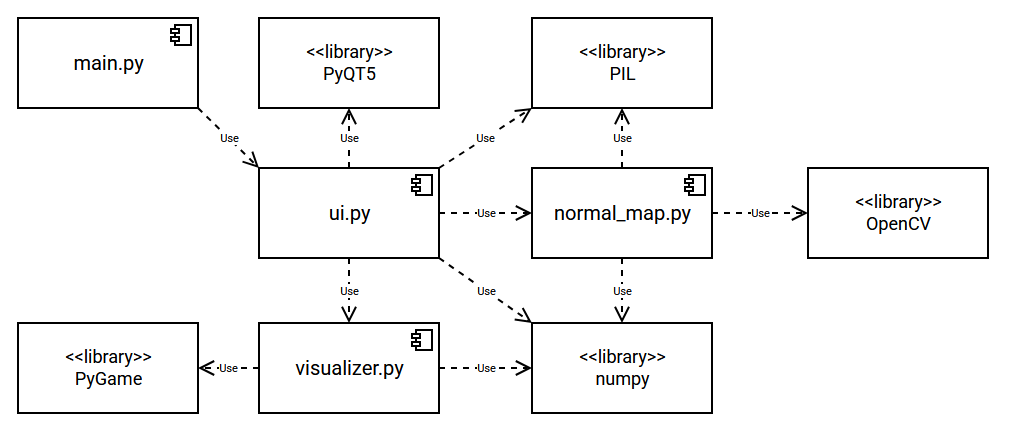
\includegraphics[width=1\linewidth]{compo}
	\caption{Диаграмма компонентов}
	\label{compo:image}
\end{figure}

Система реализована как настольное приложение с графическим интерфейсом, выполненным с использованием библиотеки PyQt5, и состоит из следующих логических компонентов:

\begin{enumerate}
	\item Интерфейсный модуль (ui.py).
	\item Модуль генерации нормалей (normal-map.py)
	\item Модуль визуализации освещения (visualize.py)
	\item Главный управляющий модуль (main.py)
\end{enumerate}
\subsubsection{Интерфейсный модуль}

Отвечает за визуальное представление программы и взаимодействие с пользователем. Основные элементы:
\begin{enumerate}
	\item Главное окно приложения с двумя основными вкладками (Генерация и Визуализация).
	\item Кнопки для загрузки, сохранения изображений, запуска генерации и визуализации.
	\item Слайдеры и переключатели, управляющие параметрами генерации и визуализации (например, сила нормалей, интенсивность света, радиус света, выбор оператора градиента и т.д.).
	\item Модуль обрабатывает действия пользователя и передаёт команды в функциональные модули системы.
\end{enumerate}

Модуль обрабатывает действия пользователя и передаёт команды в функциональные модули системы.
\subsubsection{Модуль генерации нормалей}

Реализует логику построения карты нормалей по загруженному изображению. Поддерживает несколько операторов градиентного анализа:
\begin{itemize}
	\item Sobel;
	\item Scharr;
	\item Prewitt.
\end{itemize}

Дополнительно реализована возможность настройки:
\begin{itemize}
	\item силы нормалей (интенсивность отклонения векторов нормали);
	\item глубины нормалей (масштаб значения градиента по оси Z);
	\item инверсии направления нормалей (для совместимости с разными движками).
\end{itemize}

Результатом работы модуля является изображение, где RGB-каналы кодируют направления нормалей в пространстве.
\subsubsection{Модуль визуализации освещения}

Отвечает за отображение эффекта освещения текстуры с наложенной картой нормалей. Основные особенности:
\begin{enumerate}
	\item Механизм "фонарика" — направление света зависит от положения курсора мыши.
	\item Параметры освещения — интенсивность и радиус света настраиваются пользователем.
	\item Рендеринг результата — на лету пересчитывается яркость пикселей, имитируя взаимодействие света с поверхностью, представленной нормалями.
\end{enumerate}

Визуализация реализована вручную без использования графических движков, что демонстрирует работу с нормалями "на низком уровне".
\subsubsection{Главный управляющий модуль}

Запускает интерфейс приложения, инициализирует все компоненты, связывает обработчики интерфейса с функциональными модулями.
\subsection{Реализация модуля генерации карт нормалей}

Модуль генерации карт нормалей представляет собой ключевую компоненту программной системы, предназначенную для преобразования обычного двухмерного изображения в нормал-карту — трёхканальное изображение, содержащее информацию о направлении нормалей к виртуальной поверхности. Это позволяет имитировать рельефность изображения без использования дополнительных геометрических деталей [27].

Процесс генерации карты нормалей состоит из нескольких последовательных этапов.

На первом этапе входное изображение преобразуется в оттенки серого. Это необходимо для упрощения дальнейшего анализа, поскольку данные о цвете не участвуют в расчётах нормалей. Затем изображение конвертируется в числовой массив, содержащий значения яркости каждого пикселя.

Далее производится вычисление градиентов изображения — то есть изменений яркости по горизонтали и вертикали. Для этого применяется один из операторов свёртки: Sobel, Scharr или Prewitt. Пользователь может выбрать нужный оператор через интерфейс. Эти операторы позволяют определить, насколько сильно и в каком направлении изменяется яркость изображения в каждой точке. Это изменение отражает структуру "высот" изображения, которую можно трактовать как рельеф.

Полученные горизонтальные и вертикальные градиенты масштабируются в соответствии с заданным пользователем параметром силы нормали. Чем выше значение силы, тем контрастнее будет рельеф на итоговой карте нормалей.

Третья компонента нормали, направленная перпендикулярно изображению (в глубину), задаётся как фиксированное значение, также масштабируемое по параметру глубины. Далее на основе трёх компонентов (по осям X, Y и Z) формируется вектор нормали. Все векторы нормализуются, то есть приводятся к единичной длине, чтобы сохранить корректность направлений.

При необходимости пользователь может включить параметр инверсии, при котором направление векторов нормалей меняется на противоположное. Это может быть полезно для корректной работы с различными движками визуализации, ожидающими ту или иную ориентацию нормалей.

В завершение формируется итоговая нормал-карта. Она состоит из трёх каналов, соответствующих осям X, Y и Z, и преобразуется в формат, пригодный для отображения и сохранения (все значения нормалей переводятся из диапазона [-1; 1] в [0; 1]). Итоговое изображение возвращается в виде массива и может быть использовано в визуализации или сохранено на диск.

Таким образом, реализованный модуль генерации карт нормалей позволяет на основе 2D-изображения создавать полноценную нормал-карту, пригодную для последующего освещения и анализа микрорельефа. Применение градиентных операторов в сочетании с настраиваемыми параметрами обеспечивает гибкость и точность работы алгоритма.
\subsection{Реализация модуля визуализации освещения}

Модуль визуализации освещения предназначен для интерактивного отображения рельефа изображения, сгенерированного на основе карты нормалей. Основной задачей является имитация динамического света, который пользователь может перемещать в реальном времени, наблюдая, как он влияет на освещённость различных участков изображения [28].

В основе визуализации лежит физическая модель освещения, имитирующая точечный источник света ("фонарик"), направленный на плоскую поверхность с заданными нормалями. Каждая нормаль определяет, в каком направлении ориентирована виртуальная поверхность в данной точке изображения. Сравнивая направление нормали и направление света, можно рассчитать яркость в данной точке с помощью скалярного произведения.

После запуска модуля создаётся графическое окно с помощью библиотеки pygame, в котором отображается результат освещения. Размер окна соответствует разрешению карты нормалей.

Затем выполняется преобразование нормалей из диапазона [0, 1] в стандартный векторный диапазон [-1, 1]. Это необходимо, чтобы работать с корректными векторными направлениями.

Если пользователь не загрузил исходное изображение, для подсветки используется равномерный серый фон. Иначе применяется оригинальное изображение, масштабированное под размер нормал-карты.

Основной цикл визуализации обрабатывает положение мыши как координаты источника света. Для каждой точки изображения рассчитывается вектор от пикселя к источнику света. Этот вектор нормализуется, после чего по скалярному произведению с нормалью определяется уровень освещения.

Результат также модифицируется с учётом радиуса действия света (затухание по расстоянию) и фоновой освещённости (ambient). 

Полученное значение освещённости используется для модификации яркости пикселя оригинального изображения.

Таким образом, визуализация реализует освещение Lambertian-модели: чем больше угол между направлением света и нормалью, тем слабее освещённость.

При закрытии окна происходит корректное завершение всех процессов библиотеки pygame. Это позволяет избежать зависаний или конфликтов при повторном запуске визуализатора в рамках одного сеанса работы программы.

Таким образом, реализованный модуль визуализации обеспечивает наглядную демонстрацию эффекта нормалей на освещённость изображения. Благодаря интерактивному управлению пользователем и моделированию точечного света достигается реалистичное ощущение глубины и рельефа, что значительно расширяет возможности анализа и применения нормал-карт.
\subsection{Структура пользовательского интерфейса}

На основании требований к пользовательскому интерфейсу [19], представленных в пункте 2.3.2.1 технического задания, был разработан графический интерфейс приложения. Интерфейс реализован с использованием библиотеки PyQt5, которая позволяет создать графическое приложение с гибкой системой компоновки элементов и поддержкой событий.

Интерфейс программы представлен на рисунке ~\ref{interf:image}.

\begin{figure}[ht]
	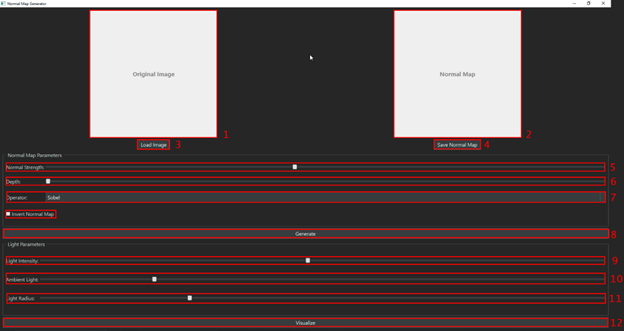
\includegraphics[width=1\linewidth]{interf}
	\caption{Интерфейс программы}
	\label{interf:image}
\end{figure}

Элементы интерфейса:
\begin{enumerate}
	\item Окно оригинального изображения. Отображает исходное изображение, загруженное пользователем для генерации карты нормалей.
	\item Окно карты нормалей. Показывает сгенерированную карту нормалей на основе оригинального изображения и выбранных параметров.
	\item Кнопка "Load Image". Открывает диалоговое окно выбора изображения, которое будет использоваться для анализа и генерации нормалей.
	\item  Кнопка "Save Normal Map". Сохраняет сгенерированную карту нормалей в выбранное пользователем место.
	\item Ползунок "Normal Strength" (Сила нормалей). Регулирует интенсивность/амплитуду нормалей. Чем выше значение, тем рельефнее выглядит результат.
	\item Ползунок "Depth" (Глубина). Активирует дополнительное влияние глубины на расчет нормалей (если предусмотрена соответствующая логика в коде).
	\item Выпадающий список "Operator". Позволяет выбрать математический оператор, применяемый для выделения границ (например, Собель, Шарра и др.).
	\item Чекбокс "Invert Normal Map" (Инвертировать нормали). При включении инвертирует направление нормалей, меняя визуальное восприятие рельефа.
	\item Ползунок "Light Intensity" (Интенсивность света). Управляет яркостью источника света при визуализации эффекта освещения.
	\item Ползунок "Ambient Light" (Фоновое освещение). Добавляет равномерное базовое освещение всей сцены для повышения читаемости изображения.
	\item  Ползунок "Light Radius" (Радиус освещения). Определяет зону, охватываемую виртуальным "фонариком". Чем больше значение, тем шире область освещённости.
	\item Кнопка "Visualize" (Визуализировать). Активирует режим визуализации, в котором курсор мыши используется как источник света для динамического освещения по карте нормалей.
\end{enumerate}
